\documentclass[man,floatsintext]{apa7}
\usepackage[american]{babel}
\usepackage{csquotes}
\usepackage{microtype}
\usepackage{mathtools}
\usepackage{booktabs}
\usepackage{graphicx}
\usepackage{hyperref}
\hypersetup{pdftitle={When the True Controller Is Not Recoverable: Observational Equivalence in Models of Relational Regulation},pdfauthor={Mateusz Pomianek}}
\usepackage[style=apa,sortcites=true,sorting=nyt,backend=biber]{biblatex}
\addbibresource{references.bib}

\title{When the True Controller Is Not Recoverable: Observational Equivalence in Models of Relational Regulation}
\shorttitle{Regulatory Model Identifiability}
\authorsnames{Mateusz Pomianek}
\authorsaffiliations{Rzeszów University of Technology}
\abstract{Distinct dynamical mechanisms can predict similar actions, so family recovery, predictive accuracy and practical loss equivalence must be evaluated separately. We examine these distinctions using synthetic feedback trajectories. Historical ARC-inspired stress tests motivate the problem but are not confirmatory evidence. A standardized development benchmark crosses six two-level observation factors with eight generator families, producing 40,960 trajectories with separate fitting, validation choice and final evaluation. A further 5,760 targeted trajectories include exact reduction of PID to P. In the full grid's reference arm, nominal PID recovery was 79/80; analyst-noise SD 0.04 reduced it to 41/80. High family recovery could coexist with predictive loss differences inside the development tolerance. Short and sparse observation schedules also left 2,432 attempts without enough observations, which remain in recovery denominators. A further exploratory extension generated 26,880 trajectories for independent-role validation, AIC/BIC comparison and observation stress tests. Penalization improved recovery of simpler nested labels but could reduce noisy PID recovery; bootstrap conclusions remained strongly tolerance-dependent. These development results establish conditional design sensitivity within a specified generator universe, not structural equivalence or human mechanisms. Final inferential claims require calibrated tolerance, precision planning and independent reproduction of a frozen numerical protocol.
}
\keywords{system identification, practical identifiability, observational equivalence, dynamical models, regulatory behavior, simulation}

\begin{document}
\maketitle
\section{Scope and Motivation}

This methodological manuscript asks whether latent regulatory mechanisms can be identified from noisy, discretely sampled action trajectories. Attachment-related regulation provides the motivating application, but the methodological claim is broader than attachment theory. P, PI, and PID are treated as deliberately simple benchmark generators rather than privileged psychological mechanisms.

System identification requires more than fitting a plausible trajectory. A model family can predict well while its parameters or mechanism remain practically non-identifiable, especially under limited data, measurement error, feedback, nonlinear saturation, and partial observation \parencite{ljung1999systemidentification,lam2022identifiability}. This distinction is critical when model labels are interpreted psychologically.

The paper therefore separates three questions: whether a model predicts held-out behavior; whether the correct generating family can be recovered; and whether parameters within a selected family are estimated with useful precision. Failure on the second or third question limits mechanistic interpretation even if the first question is satisfactory.

\section{Identifiability Problem}

Let an observed action sequence be $\mathbf y=(y_1,\ldots,y_T)$ and let $\mathcal M_k$ denote a candidate model family with parameters $\theta_k$. Prediction identifies a model that minimizes an out-of-sample loss,
\[
\hat{k}=\arg\min_k L_{\mathrm{val}}(\mathcal M_k,\hat\theta_{k,\mathrm{fit}}),
\]
but a small loss difference does not imply that the generating family is uniquely recoverable.

Model choice is frozen before computing final-test loss; the test block never determines $\hat{k}$. Family recovery is agreement between the validation-selected family and the known synthetic generator. Final evaluation estimates predictive performance of that frozen choice, not a second opportunity to select a family.

For replicate $j$, let $\Delta_j=L_{\mathrm{test},j}(\mathcal M_k)-L_{\mathrm{test},j}(\mathcal M_l)$ for a comparison specified before final evaluation. A trajectory-level near tie is $|\Delta_j|<\epsilon$. Its frequency describes practical ambiguity but does not establish statistical equivalence. At the observation-condition level, equivalence is supported only if the prespecified confidence interval for the mean paired difference lies wholly within $[-\epsilon,\epsilon]$. An interval crossing a boundary is inconclusive; a nonsignificant superiority test does not establish equivalence. The tolerance, loss scale, interval method, coverage level, and comparison family remain pending prospective freeze in \texttt{simulation\_protocol.yaml}. This is practical predictive equivalence within the investigated model universe, not structural equality of mechanisms.

Feedback creates a difficult setting because action changes future state. Competing controllers can therefore drive the system toward similar regions even when their internal terms differ. Clipping and policy gating compress observable differences further. Measurement noise affects the analyst's reconstructed discrepancy, while missing observations alter numerical estimates of integral and derivative terms.

Non-identifiability is treated as a substantive result. If a simple baseline or lower-order model is predictively indistinguishable from a richer model, the available observation design does not warrant the richer mechanistic label.


\subsection{Three Distinct Definitions}

\paragraph{Observational equivalence.}
Let $\mathcal O_T=\{(t_i,\widetilde e_i,\widetilde a_i)\}_{i=1}^{m(T)}$ be the observed record under design $\mathcal D$, including sampling, omission and measurement rules. Two parameterized generators are observationally equivalent under that design when their induced observation laws agree:
\[
\mathsf P^{\mathcal D}_{k,\theta_k}(\mathcal O_T\in B)
=\mathsf P^{\mathcal D}_{l,\theta_l}(\mathcal O_T\in B)
\quad\text{for every measurable }B.
\]
Equivalence for a restricted observation design is weaker than equivalence over all admissible designs and durations. A small empirical loss difference does not establish equality of these probability laws. Exact PID reduction to P is a separate algebraic case: with $k_I=k_D=0$ and matched initial conditions and innovations, the action/state recursion is identical. Different nominal family labels can therefore represent the same mechanism.

\paragraph{Practical predictive equivalence.}
For independently generated replicate units, define
\[
\Delta_j=L_j(\widehat{\mathcal M}_{k,\mathrm{fit}})
-L_j(\widehat{\mathcal M}_{q_j,\mathrm{fit}}),
\qquad \mu_\Delta=\mathsf E[\Delta_j],
\]
where $q_j$ is chosen before final evaluation and excludes the nominal generating family. It may differ across replicates. The estimand concerns fitted predictions and this competitor-selection rule, not an oracle comparison of latent equations. For a positive tolerance $\epsilon$, practical mean-loss equivalence means $|\mu_\Delta|<\epsilon$; the operational development rule requires interval containment within $[-\epsilon,\epsilon]$. This neither entails observational equivalence nor validates a psychological mechanism.

\paragraph{Family recovery.}
For $N$ attempted replicate units with nominal generator $k$, the empirical recovery rate is
\[
\widehat R_k(\mathcal D)=\frac{1}{N}\sum_{j=1}^{N}
\mathbf 1\{\widehat k_j=k\}.
\]
Failed selections contribute zero. Recovery over evaluable units is additionally reported with its own denominator. Effective-family recovery replaces $k$ with an explicitly defined reduction label; a practical nonzero-gain threshold is not inferred from the observed winners. Within-family parameter identification, family-label recovery and predictive equivalence remain distinct questions.

\section{Current Synthetic Evidence}

\subsection{Original stress test}

The original generator-discrimination experiment generated 40 trajectories for each of P, PI, and PID using matched gain distributions and random seeds across generator families. Each trajectory was fitted with intercept-only (labeled context in code), autoregressive, P, PI, and PID alternatives. Analyst discrepancy-measurement noise was evaluated at SD 0 and 0.04.

Without added analyst measurement noise, the generating nested family was selected in 20/40 P trajectories, 11/40 PI trajectories, and 14/40 PID trajectories. With measurement-noise SD 0.04, correct selections fell to 13/40, 7/40, and 6/40. Under the noisy arm, a simple baseline had the lowest error in 32/40 trajectories for each generator condition.

These results are descriptive rather than confirmatory. The same final 30\% chronological block was used both to choose the model and to describe its holdout performance, so selection accuracy is entangled with performance reporting. The evidence is retained as \texttt{M02-STRESS-TEST-LEGACY} and used only to motivate the identifiability problem.

\subsection{Leakage-resistant development benchmark}

A revised development pipeline separated coefficient fitting (60\%), validation/model selection (20\%), and untouched final evaluation (20\%). The generator set remained P/PI/PID, while candidates included intercept-only (labeled context in code), autoregressive, P, PI, and PID models. Forty trajectories per generator were evaluated at analyst-noise SD 0 and 0.04. This run is registered as \texttt{M02-DEV-SPLIT-2026-10-01}; it verifies analysis architecture but does not freeze the confirmatory design.

\begin{table}[htbp]
\centering
\caption{Leakage-resistant development benchmark: validation-selected family recovery}
\begin{tabular}{llrrrr}
\toprule
Generator & Noise SD & $n$ & Nested correct & All-candidate correct & Baseline selected \\
\midrule
P   & 0.00 & 40 & 19 & 19 & 0 \\
PI  & 0.00 & 40 & 12 & 12 & 2 \\
PID & 0.00 & 40 & 11 & 11 & 1 \\
P   & 0.04 & 40 & 10 & 0  & 36 \\
PI  & 0.04 & 40 & 8  & 1  & 39 \\
PID & 0.04 & 40 & 14 & 0  & 37 \\
\bottomrule
\end{tabular}
\end{table}

Separating model selection from final evaluation did not eliminate the ambiguity. In the zero-noise arm, correct all-candidate selection ranged from 11/40 to 19/40 across generators. With analyst-noise SD 0.04, the generating family was selected from the full candidate set in only 1 of 120 trajectories, whereas a intercept-only (labeled context in code) or autoregressive baseline was selected in 112 of 120. Mean final-test RMSE of the validation-selected model was also lower than that of the true generating family in the noisy arms, indicating that the observable action sequence can favor a simpler predictive explanation even when the simulator's latent generator is known.

This is a development result, not the manuscript's final inferential result. The candidate universe is still narrow, the factor grid is not frozen, and the practical-equivalence tolerance has not been prespecified. The confirmatory study therefore expands generator classes and observation conditions, freezes the numerical grid and equivalence criterion before execution, and reports Monte Carlo uncertainty on untouched final evaluation data.

\section{Standardized Closed-Loop Development Experiment}

To separate observation-design effects from the additional gating and trait-dependent terms of the historical ARC-inspired simulator, a second benchmark uses a standardized dimensionless feedback plant. This complements the previous simulator; it neither replaces ARC nor represents a fitted model of people. At unit latent time steps,
\[
 e_t=r_t-x_t,\qquad x_{t+1}=x_t+b a_t+\eta_t,\qquad
 a_t=\operatorname{clip}\{f_k(e_{\leq t},a_{<t})+\xi_t,-A,A\}.
\]
The target $r_t=0.12\sin(t/13)+\zeta_t$ provides persistent excitation. Independent Gaussian target, process and action noise have SD 0.04, 0.003 and 0.005, respectively. These are computational settings, not calibrated human measurement properties. The plant state is not clipped. Feedback strength $b$ and action bound $A$ are design factors.

The eight generators are zero-intercept noise, AR(1), P, PI, PID, ARX, a fixed-width hyperbolic-tangent response and a sign-dependent switching-slope response. The controller regressors use $I_t=0.85I_{t-1}+e_t$ and $D_t=e_t-e_{t-1}$, initialized at zero. Regular gains are $k_P=0.6$, $k_I=0.06$, $k_D=0.08$; AR persistence is 0.65, nonlinear amplitude is 0.15 with width 0.12, and positive/negative switching slopes are 0.75/0.25. The switching boundary is the known discrepancy zero, not an estimated hidden regime. Knowing nonlinear width and switching boundary is an optimistic benchmark assumption.

Candidates are an intercept-only model, observed-lag AR, P/PI/PID, ARX, fixed-width nonlinear regression and sign-dependent slopes, all fitted by ordinary least squares with an intercept. Additive action noise precedes clipping. Consequently, clipped conditions deliberately violate an unclipped linear candidate equation. Estimated regression coefficients under clipping or noisy reconstructed history need not recover latent generator gains. Parameter summaries retain this distinction and do not report unavailable interval coverage.

\begin{table}[htbp]
\centering
\caption{Two-level observation-factor grid for the standardized development study}
\label{tab:m02-development-design}
\begin{tabular}{ll}
\toprule
Factor & Levels \\
\midrule
Latent trajectory steps & 60, 180 \\
Observation stride & 1, 3 latent steps \\
Analyst discrepancy-noise SD & 0, 0.04 \\
MCAR omission probability & 0, 0.25 \\
Feedback coefficient $b$ & 0.1, 0.5 \\
Symmetric action bound $A$ & 0.025, 1.0 \\
\bottomrule
\end{tabular}
\end{table}

The full development design crosses these six factors: 64 observation conditions, eight generators and 80 independent seed blocks per cell. A separate targeted study contains nine conditions, including exact PID reduction to P, and uses a different seed pool. Seed streams are matched across generator families and condition contrasts. Factorial and targeted results remain separate development evidence, with no claim of prospective external registration or a confirmatory psychological tolerance.

Observations retain time zero, remove MCAR snapshots and add discrepancy measurement noise. Derivative/integral features use actual elapsed time and retained observations, without interpolation or hidden latent histories. After gaps, autoregression uses the previous observed action; this is not the previous latent-step action. Temporal 60/20/20 blocks are defined after observation processing. Full-rank candidates are fitted on the first block; exact ties in validation RMSE follow the fixed candidate order. Rank-deficient/numerically failed candidates and trajectories with insufficient observations remain in the ledger. The best competitor excludes the nominal generating family and is frozen on validation. Only after these choices are frozen are final-block actions used to compute losses.

Recovery intervals use Wilson 95\% intervals with attempted trajectories as denominators. Paired mean-loss intervals use a pointwise normal approximation over independent seed blocks. The development equivalence band is $\epsilon=0.005$ in action-RMSE units, set before the first targeted run and retained for the full grid. It is a computational resolution choice, not a human-calibrated minimal difference. Multiple cellwise conclusions are descriptive, with no familywise confirmatory guarantee. Final-test prediction is conditional on observed current discrepancy and past observations; it is not recursive autonomous forecasting.

\section{Standardized Development Results}

The full $2^6$ observation grid generated 40,960 trajectories in 512 generator-condition cells using fresh seed blocks. Of these attempts, 2,432 lacked enough retained observations for the required split, leaving 38,528 evaluable trajectories. These attempts remain unsuccessful recovery in attempted-run summaries. There were also 672 candidate-level rank-deficient fits; candidate failures are distinct from trajectory failures and are not an additional number of excluded trajectories. These are developmental results registered as \texttt{M02-DEV-FACTORIAL-2026-10-07}.

\begin{table}[htbp]
\centering
\caption{Standardized development benchmark: nominal recovery}
\label{tab:m02-standardized-development}
\begin{tabular}{lrrr}
\toprule
Generator & Reference & Analyst noise & Combined \\
\midrule
intercept & 17/80 & 12/80 & 12/80 \\
ar & 42/80 & 46/80 & 4/80 \\
p & 15/80 & 4/80 & 1/80 \\
pi & 47/80 & 29/80 & 8/80 \\
pid & 79/80 & 41/80 & 4/80 \\
arx & 80/80 & 77/80 & 9/80 \\
nonlinear & 78/80 & 24/80 & 16/80 \\
switching & 79/80 & 40/80 & 11/80 \\
\bottomrule
\end{tabular}
\end{table}


In the referent condition (180 steps, stride 1, no analyst noise or gaps, $b=0.5$, $A=1$), nominal PID recovery was 79/80, with Wilson 95\% interval approximately 0.933--0.998. At analyst-noise SD 0.04, it fell to 41/80 (approximately 0.405--0.619). Combined adversity used 60 steps, stride 3, noise SD 0.04, MCAR probability 0.25, feedback 0.1 and action bound 0.025. PID recovery was 4/80 attempts, or 4/42 evaluable trajectories. Reporting only the latter denominator would conceal observation-design infeasibility.

Recovery also varied substantially across generators within the reference arm: P was selected in 15/80 attempts and the intercept-only generator in 17/80, compared with 79/80 for PID. The candidate set contains richer regressions that include lower-order behavior as a special case. Unpenalized validation RMSE can therefore favor a richer family even when the nominal generator is simpler. Exact nominal recovery is a demanding label-level criterion; these counts cannot by themselves establish that P-like behavior is poorly predicted. Confusion matrices and effective-order scores complement nominal recovery, and a uniform chance rate is inappropriate for this nested set.

Combined adversity did not universally favor the simplest baselines. For nominal PID in that arm, the selected families included nonlinear in 13 cases, PI in 10 and ARX in 7, but intercept in only 2 and AR in none; 38 attempts failed the observation split. Family confusion and design failure therefore require separate interpretation.

Strong nominal discrimination did not guarantee a material predictive advantage at the chosen development resolution. Reference PID's mean paired final-test RMSE difference against its validation-selected competitor was approximately $-0.000841$, with pointwise 95\% normal interval $[-0.000957,-0.000725]$. This interval excludes zero but remains inside the development band $[-0.005,0.005]$. Statistical separation from zero and practical predictive equivalence therefore coexist at this resolution; neither conclusion is structural equivalence or evidence about people.

Across the 512 cells, 405 paired mean intervals were wholly inside the development band, 74 were inconclusive, 23 favored the nominal generator beyond the band and 10 favored the competitor beyond it. These are pointwise development descriptions rather than multiplicity-controlled confirmatory decisions. Short/sparse adverse conditions can produce unstable candidate extrapolation and very broad intervals; the normal approximation and fixed numerical tolerance require further calibration before final inferential claims.

The separate targeted benchmark generated 5,760 trajectories with a different seed pool. Its exact-reduction condition gives the nominal PID generator zero integral and derivative gains. This produces actions identical to P under matched noise. Nominal PID was selected in 14/80 cases while effective P was selected in 20/80. The discrepancy between those scores is a labeling issue, not recoverable evidence for distinct mechanisms. The targeted study is registered separately as \texttt{M02-DEV-STANDARDIZED-2026-10-07}; it is not pooled with the factorial grid.

\begin{figure}[htbp]
\centering
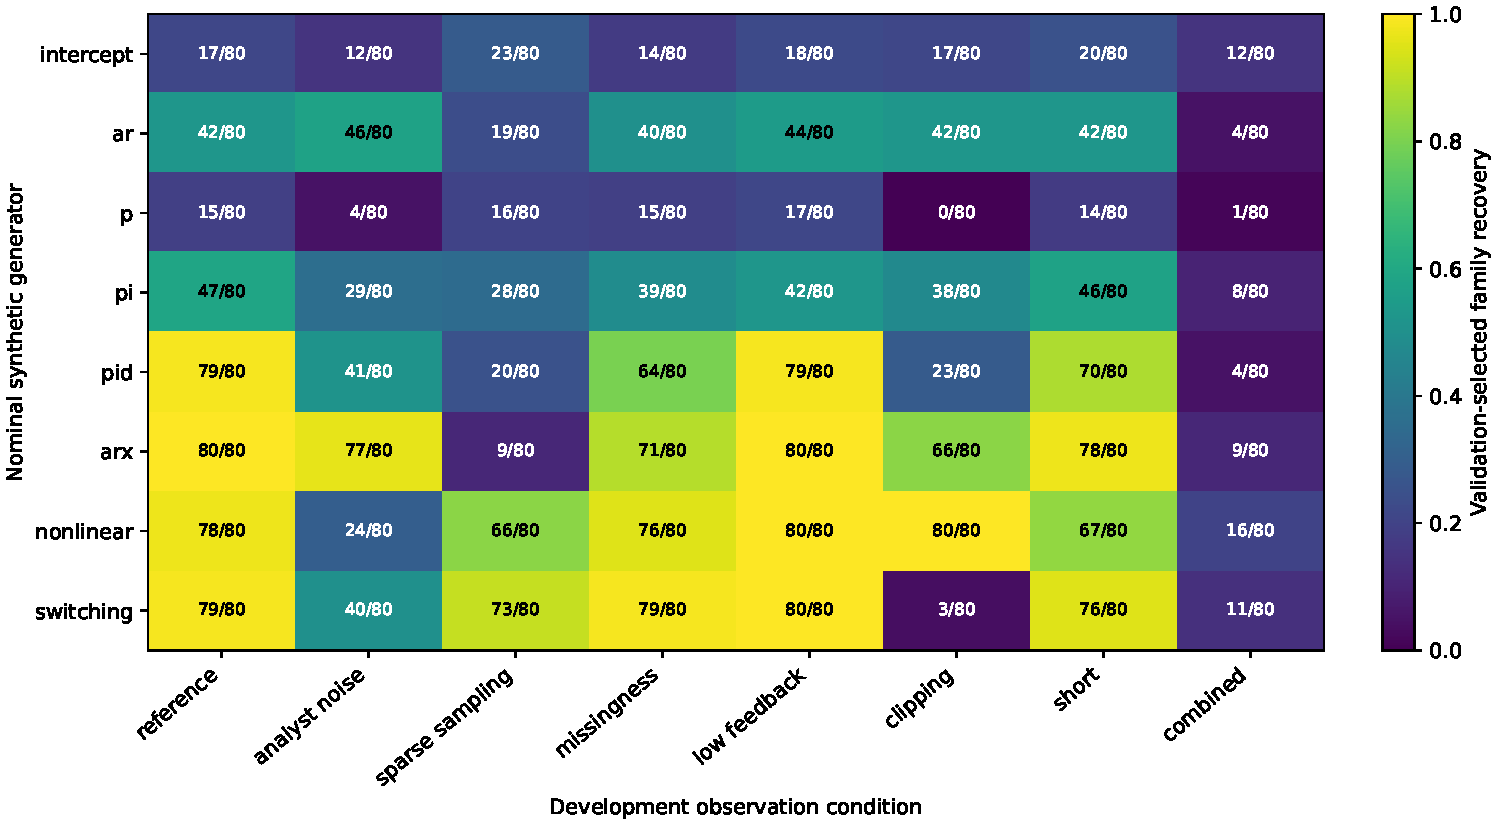
\includegraphics[width=\linewidth]{figures/m02_development_recovery.pdf}
\caption{Nominal generator recovery in eight displayed observation arms of the full development grid. Counts retain all 80 attempts per cell, including failed trajectory splits. Colors show validation-selected recovery, not psychological validity. The complete 64-condition summaries and Wilson intervals are archived separately.}
\label{fig:m02-development-recovery}
\end{figure}

\begin{figure}[htbp]
\centering
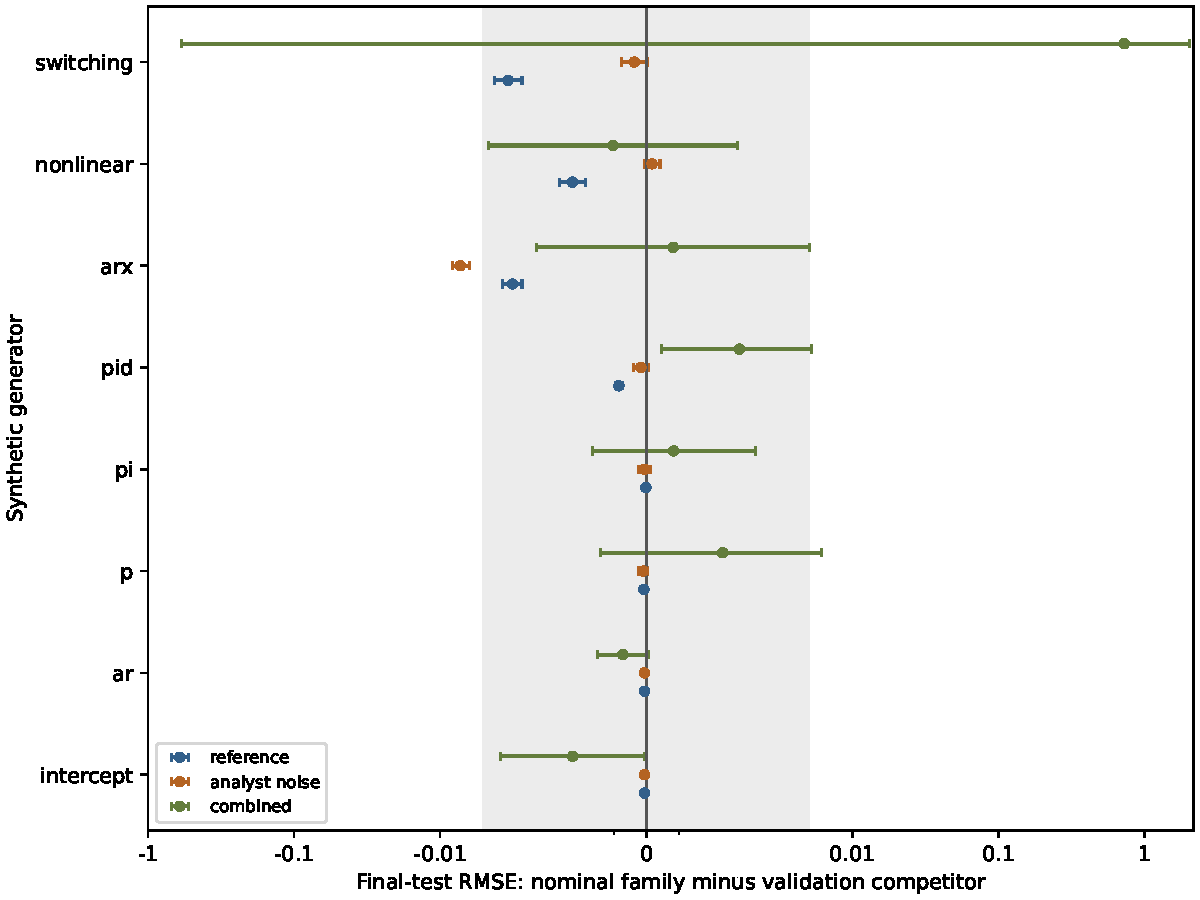
\includegraphics[width=0.90\linewidth]{figures/m02_development_paired_loss.pdf}
\caption{Paired final-test RMSE differences for three development arms. Negative values favor the fitted nominal family; positive values favor the competitor chosen on validation excluding that family. Pointwise 95\% normal intervals use evaluable paired trajectories, with counts in the archived summary. The shaded band is the fixed development tolerance; the horizontal axis is symmetric logarithmic outside its central linear region. Broad intervals are inconclusive rather than evidence of equality.}
\label{fig:m02-development-paired-loss}
\end{figure}

All generators use fixed gains, and nonlinear width and switching boundary are known. The plant deliberately simplifies the historical ARC-inspired agent. MCAR gaps, conditional action prediction and noisily reconstructed histories limit transfer beyond these settings. Parameter bias/dispersion are archived for evaluable nominal-family fits, without implemented coverage intervals. Neither development experiment substitutes for a frozen, independently reproduced final computational protocol.

\section{Exploratory Methodological Robustness}

The review-driven extension uses fresh seed streams and remains development evidence. Its settings were recorded before this new execution, after the earlier development results were known. It does not retrospectively preregister those results. There are seven targeted conditions and eight generators, with 160 independent replicate triads per cell: 8,960 triads and 26,880 generated trajectories. The standardized plant and gains remain unchanged.

\subsection{Independent Trajectories and Selection Criteria}

Each triad contains separate fitting, validation and final-test trajectories. Coefficients use only the first 60\% of retained observations of the fitting trajectory. Independent validation uses the middle 20\% of its own trajectory and independent final evaluation the last 20\% of its own trajectory, matching the temporal benchmark's scoring windows when retained counts agree. Each trajectory reconstructs its own causal feature history from its preceding observations; no state or history is transferred between roles. Thus generalization concerns fresh innovations under the same generator, gains, target schedule and observation design, with causal prehistory available. It does not test new gains, new initial-state distributions, people or autonomous forecasts. The temporal comparator reuses only the fitting trajectory's 60/20/20 windows. All three trajectories must satisfy the split requirement; failed triads remain in both designs' attempted denominators. This common feasibility gate can be stricter than a single-trajectory gate.

The extension compares validation RMSE with Gaussian working information criteria \parencite{akaike1974newlook,schwarz1978dimension}:
\[
\mathrm{AIC}=n\log(\mathrm{RSS}/n)+2q,
\qquad
\mathrm{BIC}=n\log(\mathrm{RSS}/n)+q\log n,
\]
where $n$ is the fitting count and $q$ counts all fitted regression coefficients, including the intercept, plus residual variance. Common likelihood constants are omitted. Rank-deficient fits are ineligible; nonpositive RSS has no finite working variance MLE and is unavailable for AIC/BIC. Information criteria use fitting data alone, while RMSE uses the designated validation trajectory/block. Coefficients are not refitted after selection. Each method separately freezes its best competitor excluding the nominal family before final scoring.

Nested models can improve fitting RSS by adding coefficients, but validation loss need not improve monotonically with complexity. AIC/BIC are methodological sensitivity checks, not automatic corrections of an invalid likelihood. Clipping, noisy reconstructed predictors, categories and residual dependence limit the Gaussian assumptions. BIC is not a computed Bayes factor here. Full Bayesian model selection requires specified parameter/model priors and a justified observation likelihood; it is deferred rather than approximated by relabeling BIC. Independent trajectories remove shared realized state across roles, but do not guarantee optimal model selection. A finite temporal purge cannot fully reset a feedback process with leaky memory; its adequacy would require a separate dependence analysis.

\subsection{Observation and Interval Sensitivity}

Targeted observation arms add Student-$t$ analyst noise with three degrees of freedom, scaled to the same SD 0.04 as Gaussian noise; irregular Bernoulli sampling with nominal mean stride three; and seven equally spaced categories for discrepancy and action within $[-0.25,0.25]$. Categories are converted back to their simulator-scale centers before fitting. These bounds are explicit computational choices, not validated Likert thresholds, and the transformation changes both the response and regressors. Reference, Gaussian-noise, clipping and combined-adversity arms complete the targeted design. Realized counts and elapsed intervals are retained; no interpolation is applied. Heavy-tail, irregular and quantization arms are one-factor stress tests rather than a full interaction grid or a fitted behavioral measurement model.

Paired-loss uncertainty is additionally evaluated by a percentile bootstrap with 2,000 resamples of independent replicate-level differences. Each difference retains the nominal-family and frozen-competitor losses together. Time points are never resampled as independent units. Pointwise percentile intervals offer a distribution-sensitive comparison, not guaranteed coverage with small samples or rare extreme losses. Permutation tests require a justified exchangeability or sign-symmetry null; they are not substituted automatically for mean-loss intervals. Multiplicity-controlled confirmation and interval-coverage calibration remain open.

An exploratory reanalysis of the previously inspected factorial ledger applies the same bootstrap and evaluates $\epsilon\in\{0.001,0.0025,0.005,0.01\}$. These values equal 0.2, 0.5, 1 and 2 times the latent action-innovation SD 0.005. This gives the tolerance an explicit computational scale while retaining the original pre-run value. It does not supply a human minimal important difference or license choosing the most favorable threshold. The original normal-interval results remain preserved alongside the sensitivity analysis.

\subsection{Conditional Information and Profile Diagnostics}

The extension diagnoses the PID regression with slope features $\Phi$ and an intercept nuisance term. Under a fixed-design Gaussian working model with known $\sigma=0.005$, its conditional slope information is
\[
\mathcal I_{\beta\mid\mathrm{intercept}}
=\sigma^{-2}\Phi^{\mathsf T}
\left(I-\frac{\mathbf 1\mathbf 1^{\mathsf T}}{n}\right)\Phi.
\]
Eigenvalues and conditioning after feature normalization describe local excitation and collinearity in that regression. For each coefficient, an illustrative profile fixes it and refits the remaining coefficients; the working deviance is
\[
D_i(v)=\{\mathrm{RSS}_{i,\mathrm{profile}}(v)-\mathrm{RSS}_{\min}\}/\sigma^2.
\]
Profiles for a fixed full-rank linear model with known variance are quadratic. Their width describes conditional regression precision under those assumptions, not structural identification of the latent controller. Profiles are retained for the first PID replicate of each arm as explicitly indexed diagnostics, not as representative aggregate evidence.

Profile likelihood is useful when the full parameterized observation likelihood is available \parencite{raue2009profile}. Here the predictors are held fixed while parameters vary. A latent closed-loop likelihood would also propagate gain changes through state, discrepancies, clipping and hidden/noisy histories. This stronger analysis, including boundary masses and measurement error, is not implemented. Rank loss in a finite observed feature matrix cannot by itself distinguish structural non-identifiability from limited excitation or observation-induced misspecification. No latent-gain interval coverage is claimed from these working profiles.

\section{Exploratory Robustness Results}

The extension attempted 8,960 replicate triads, generating 26,880 trajectories. The common observation gate failed for 968 triads, all in combined adversity; each generator retained 39 evaluable triads from 160 attempts in that arm. Failure requires any one of the three independent role trajectories to lack the minimum observations. These results therefore cannot be pooled with the previous single-trajectory failure rate. The complete archive is registered as \texttt{M02-DEV-ROBUSTNESS-2026-10-08}.

There were 663 candidate-level rank failures, distinct from failed triads. Seven-category observation made intercept/AR actions constant, leaving 1,920 full-rank candidate fits without a finite Gaussian variance MLE and 1,280 mode/criterion records without a selection. These records count as unsuccessful recovery; their unavailable AIC/BIC values are not replaced by an arbitrary variance floor. The latter count repeats choices across modes/criteria and is not an additional number of failed triads.

\begin{table}[htbp]
\centering
\caption{Exploratory nominal recovery under selection rules}
\label{tab:m02-robustness-selection}
\begin{tabular}{llrrrr}
\toprule
Arm & Generator & Temporal & Independent & AIC & BIC \\
\midrule
Reference & P & 26/160 & 31/160 & 97/160 & 147/160 \\
Reference & PID & 149/160 & 150/160 & 160/160 & 160/160 \\
Noise & P & 9/160 & 7/160 & 30/160 & 83/160 \\
Noise & PID & 83/160 & 85/160 & 82/160 & 34/160 \\
\bottomrule
\end{tabular}
\end{table}


Table~\ref{tab:m02-robustness-selection} compares nominal recovery. Temporal and independent columns use validation RMSE; AIC/BIC use the same fitting data and consequently have identical recovery across evaluation modes by construction. In the reference arm, independent validation selected P in 31/160 attempts versus 147/160 for BIC, while PID recovery was 150/160 versus 160/160. Under Gaussian analyst noise, BIC selected P in 83/160 attempts but PID in only 34/160, compared with 7/160 and 85/160 for independent validation RMSE. Penalization can resolve some nested-family labeling ambiguity while suppressing a noisy higher-order generator. These paired developmental counts do not establish a universally superior selector or a statistically established gain from independent validation.

Independent validation-RMSE PID recovery was 64/160 under variance-matched Student-$t$ noise, 32/160 with irregular sampling, 60/160 with seven-category quantization and 40/160 under clipping, versus 150/160 in the reference arm. Combined adversity yielded 5/160 attempts, or 5/39 evaluable triads. Non-Gaussian noise and altered observation schedules thus remain relevant stressors in this specified design. Quantized-response RMSE is on category-center units; its predictive performance cannot be read as unaltered latent-action performance.

For reference PID, the independent validation-RMSE mean paired loss difference was approximately $-0.000861$, with percentile bootstrap interval $[-0.000936,-0.000779]$. It remains within the original development tolerance. With combined adversity, the corresponding interval was approximately $[-0.010660,0.007407]$, crossing both equivalence boundaries. A bootstrap does not turn sparse, unstable extrapolation into a precise result.

\begin{table}[htbp]
\centering
\caption{Factorial sensitivity: pointwise bootstrap labels}
\label{tab:m02-robustness-epsilon}
\begin{tabular}{rrrrr}
\toprule
$\epsilon$ & Equivalent & Inconclusive & Generator & Competitor \\
\midrule
0.001 & 168 & 199 & 99 & 46 \\
0.0025 & 313 & 134 & 48 & 17 \\
0.005 & 404 & 69 & 24 & 15 \\
0.01 & 472 & 29 & 4 & 7 \\
\bottomrule
\end{tabular}
\end{table}


The factorial reanalysis classified 404/512 cells as development-equivalent at $\epsilon=0.005$ under percentile bootstrap, compared with 405/512 under the archived normal approximation. Eleven cell labels changed at that fixed tolerance across all categories. At $\epsilon=0.001$, only 168/512 were inside the band; at 0.01, 472/512 were inside. Table~\ref{tab:m02-robustness-epsilon} reports all four thresholds, including inconclusive and both directions of beyond-band separation. The overall similarity between interval methods at 0.005 does not establish coverage, and strong tolerance sensitivity precludes a threshold-independent equivalence claim.

PID fitting matrices were full rank in all evaluable extension triads. Median conditioning after slope-feature normalization was approximately 3.81 in the reference arm, 3.75 with Gaussian analyst noise and 7.48 in combined adversity. Full rank and modest conditional conditioning can coexist with failed family recovery: local precision conditional on noisy reconstructed inputs is not accurate recovery of latent gains. The indexed working profiles diagnose a fixed-design regression only. They do not distinguish structural non-identifiability of the closed-loop generator from measurement-induced bias.

The extension and factorial reanalysis retain their exploratory status. Fresh seeds and untouched final scoring strengthen the evaluation design, but do not undo prior knowledge of the development findings or provide a new preregistered confirmation.

\section{Prospective Confirmatory Design}

The confirmatory computational study is specified in \texttt{simulation\_protocol.yaml}. The design varies generator family, trajectory length, observation interval, analyst-side measurement noise, missingness, feedback strength, and action clipping.

The completed development grid is reported above. A separate confirmatory numerical grid and replication count will be frozen before its execution. Development runs may diagnose numerical stability and computational feasibility, but their outcomes may not be used to tune thresholds toward a preferred conclusion. Replication planning must address Monte Carlo precision, particularly in cells with observation failures or unstable paired losses.

For each generated trajectory, data are partitioned into model-fitting, model-selection/validation, and final-evaluation components. Model choice is completed without access to the final component. Family recovery is computed from the frozen validation choice and synthetic generator label; predictive losses are evaluated on the untouched final block. Random seeds, configuration hashes, software versions, and output checksums are archived.

The comparison set includes deliberately simple baselines because identifiability is scientifically relevant only relative to plausible simpler explanations. A complex controller offers little additional predictive resolution if an intercept-only or autoregressive model reproduces observable actions within the prespecified practical tolerance. That finding alone does not establish failed generating-family recovery.

The development implementation uses contiguous 60/20/20 temporal blocks of each trajectory. Temporal blocks remain statistically dependent through feedback and causal histories. Independent generated trajectories, rather than time points or blocks, define Monte Carlo replication. The exploratory extension implements separate role trajectories with fresh innovations under the same fixed generator settings. Generalization to new parameter or initial-state distributions remains a distinct prospective design.

\section{Estimands and Confirmatory Extension}

The primary estimand is generating-family recovery probability under each observation condition. Recovery is evaluated separately for the full candidate set and the nested P/PI/PID subset.

A second estimand is the paired final-evaluation loss difference between the generating-family fit and a competitor selected on validation data, excluding the generating family. The competitor and its parameters are frozen before final evaluation. Separate prespecified pairwise comparisons retain all investigated families; selecting the strongest competitor using final-test error is prohibited. Intervals use independent generated trajectories as the replication unit. If seeds are matched across conditions, resampling preserves the matched seed block. Time points within one trajectory are not independent Monte Carlo replications.

A third estimand is the trajectory-level near-tie probability under a fixed absolute loss-difference tolerance. Condition-level equivalence conclusions additionally require interval containment, as defined above; the two quantities must not share an ambiguous label. The standardized development suite implements these quantities with the pointwise intervals described in its Methods. Confirmatory comparison families, interval coverage, multiplicity handling, effective-order thresholds and loss normalization still require a prospective freeze. Repository specifications do not constitute external preregistration.

Where parameters have a meaningful generating value, the study will report bias, dispersion and interval coverage. These parameter outcomes are secondary to family-level identifiability because precise estimation within the wrong family is not mechanistic recovery.

The analysis will also estimate how family recovery changes with measurement noise, missingness, trajectory length and sampling design. Interactions are interpreted as design sensitivity rather than psychological effects.

No single winner rate will be presented without its denominator, uncertainty and competing-baseline performance. Failed fits and numerical pathologies remain in the run ledger and are summarized rather than silently discarded. Report family recovery over all attempted trajectories, with unsuccessful selections counted as unsuccessful recovery, and additionally over evaluable trajectories. Paired-loss summaries report the number evaluable for both candidates; they do not replace the attempted-run denominator. Numerical failures, insufficient observations, and near ties are separate statuses. No blanket chance rate is appropriate when candidates are unequally nested or failures alter selection opportunities; any chance benchmark must specify its random-selection rule and eligible candidate set.



The primary implemented predictive target is conditional one-step action prediction given observed discrepancy history and, for the autoregressive candidate, past observed action. A recursive multi-step rollout is a different estimand and is not implemented by the current design. Report that distinction explicitly.

Nominal-family recovery and effective-order recovery must be distinguished for nested models with zero integral or derivative gains. Nonzero gains may also be practically uninformative when regressors lack excitation or clipping dominates. The development ledger exports feature rank, conditioning, generating gains and clipping fraction; exact zero-gain reduction is implemented. A defensible rule for practically negligible nonzero gains remains open. A confidence interval wholly beyond either equivalence boundary supports predictive separation in the indicated direction; an interval crossing a boundary is inconclusive, and an interval wholly inside the band supports only practical predictive equivalence.

\section{Falsification and Reporting Rules}

The richer model hierarchy is not supported merely because PI or PID occasionally has the lowest RMSE. Generating-family recovery concerns frozen validation choices on independent synthetic replicates; final-test predictive advantage is a separate outcome. High family recovery can coexist with practically small loss differences. Conversely, low recovery need not imply poor prediction. Neither a nominal winner nor predictive equivalence alone establishes structural identifiability.

The study reports weak family recovery, simpler-baseline selection, uncertain parameter estimation and practical predictive equivalence separately. A chance benchmark requires a stated candidate-eligibility and random-selection rule. Rank failure, insufficient observations and parameter degeneracy remain explicit design/numerical outcomes. These findings restrict interpretation in the investigated generator universe rather than refuting a human mechanism.

The manuscript will not map P, PI, or PID outcomes onto attachment categories or infer human mechanisms from synthetic recovery. Human scale validation and longitudinal observations belong exclusively to M03 and M04.

\section{Reporting and Reproducibility}

The reported experiments are development evidence. Their compact archives contain immutable configuration snapshots, cellwise recovery and paired-loss summaries, confusion matrices, parameter summaries and metadata linking source, environment and output hashes. The complete trajectory-level ledger is regenerated from the documented commands rather than stored as a large repository file. It retains failed attempts and candidate diagnostics. Tables and figures are generated from these archives; the final confirmatory output contract remains in \texttt{RESULTS\_PLAN.md}.

A repeated execution of the full grid in the same Python/NumPy environment reproduced the configuration, summary, confusion, parameter and trajectory-ledger hashes byte for byte. This checks deterministic reproducibility in that environment, not independence of implementations or environments. The execution used Python 3.12.14 and NumPy 2.3.5, recorded in metadata; reproduction under the repository's locked environment remains a separate gate. No human observations were generated or analyzed.


\subsection{Local Windows Collection Audit}

A further local Windows execution of the targeted development grid produced
three collection directories containing 5,760 trajectory records each. File
manifests passed SHA-256 checks and all three directories contained
identical trajectory-level records. Consequently, these archives represent
one unique set of 5,760 developmental attempts, not 17,280 independent
replications. Their differing source-commit metadata are not evidence of
independent Monte Carlo streams.

Within the unique targeted dataset, nominal generating-family recovery was
2,988/5,760 (51.9\%), and all 5,760 attempts had a selected model and a
paired-loss contrast. Under the exploratory trajectory-level tolerance
$\epsilon=0.005$, 5,207/5,760 (90.4\%) paired differences were near ties.
This fraction must not be interpreted as the proportion of cells whose mean
losses are statistically equivalent. The combined-adversity observation arm
yielded 118/640 (18.4\%) nominal correct labels across the eight generator
families. These counts are descriptive repetitions of the previously
reported targeted experiment, not an additional confirmatory dataset.
A provenance and deduplication audit is provided in
\texttt{LOCAL\_COLLECTION\_AUDIT\_2026-10-08.md}.

\section{Observation Model and Computational Ethics}

The study uses exclusively synthetic states and actions. It recruits no participants, administers no questionnaires, and makes no individual diagnoses. No ethics approval or institutional exemption is claimed without a documented determination. Human protocols, consent, and measurement instruments belong to the separate M03 and M04 programmes.

The observation model separates latent simulator state, generator-side perception noise, process noise, and analyst-side observation error. Their scales and injection points must be recorded separately. Analyst noise is not questionnaire reliability. Numerical units in the simulator are not calibrated units of human closeness or control.

In the development pipeline, model coefficients are fitted on the first temporal block, family choice uses the next block, and final-test loss uses the last block. These are temporally ordered blocks of one feedback trajectory, not independent trajectories. Lagged observed action and causal error histories support conditional one-step prediction; they do not establish autonomous multi-step forecasting. Integral and derivative histories may cross a split boundary only through past observed information, with a documented initialization rule and no future-dependent filtering. Coefficients and preprocessing choices remain frozen for final evaluation.

Recoverability concerns the specified generator and candidate universe. It cannot establish that a corresponding mechanism or stable trait exists in people. Clipping and zero-gain cases require separate reporting because a nominal PID label may represent a functionally lower-order controller. Public computational artifacts contain synthetic data and provenance only.

\section{Discussion}

The motivating result is not that one controller family is superior. It is that feedback-regulated trajectories may contain insufficient information to identify the mechanism that generated them. This has direct consequences for computational psychology: mechanistic labels can become more specific than the observations that support them.

The standardized development grid shows that weak recovery is not universal: richer families can be recovered under favorable observation conditions, while sparse or noisy observations undermine discrimination. Nominal recovery and practical predictive value are separate axes rather than interchangeable definitions of identifiability. The final numerical protocol is intended to turn these developmental boundaries into independently reproduced inferential estimates. If richer models become recoverable only under dense, low-noise sampling, that finding informs human study design. If their predictive losses remain practically equivalent, that favors simpler predictive use at the stated resolution but does not alone establish non-identifiability of the generating family. Weak family recovery and uncertain parameters require their own evidence before restricting mechanistic interpretation.

This perspective clarifies the relationship to ARC. The ARC framework does not depend on P/PI/PID or any other controller family as a psychological type. M02 asks when latent dynamical labels are recoverable at all and therefore constrains mechanistic interpretation without serving as a prerequisite for ARC.

The local Windows repeat additionally shows that archive count must not be confused with statistical replication: three fully checksum-verified collections contained the same 5,760 trajectory records. The targeted aggregate nominal recovery (51.9\%) and trajectory-level near-tie fraction (90.4\% for the developmental tolerance) are descriptive, not multiplicity-controlled evidence for equivalence. They highlight the need to differentiate recovery, small predictive contrasts, and formal interval-contained practical equivalence.

Limitations include dependence on the chosen generator set, practical-equivalence tolerance, simulator dynamics, and observation process. A Monte Carlo study can expose ambiguity within the investigated model universe but cannot prove that all plausible mechanisms have been considered.


\subsection{Relational Motivation and Measurement Implications}

The application to relationships motivates observation design rather than validating a controller interpretation. In a dyad, both partners act and influence each other's subsequent state; the present single-plant feedback coefficient aggregates environmental response and does not estimate reciprocal co-regulation. The following implications are hypotheses for measurement design, not observed human findings.

\begin{table}[htbp]
\centering
\caption{Relational hypotheses motivating future observation design}
\label{tab:m02-relational-implications}
\begin{tabular}{p{0.21\linewidth}p{0.33\linewidth}p{0.33\linewidth}}
\toprule
Candidate process & Observation consequence & Measurement implication \\
\midrule
Reciprocal recovery & Stable feedback may narrow the range of observable discrepancy & Observe both partners and external disturbances; low variation need not mean weak regulation \\
Brief reactivity & Responses may occur between widely spaced prompts & Record timing and event-linked observations; sparse samples can alias fast changes \\
Unobserved regulatory channels & Similar recorded communication can coexist with different internal or overt actions & Separate perceived state, desired state and action channels; low observed action does not identify emotional suppression \\
\bottomrule
\end{tabular}
\end{table}

These possibilities explain why richer ecological measurements may be necessary, but a favorable synthetic design cannot guarantee psychological identifiability. M03 must establish defensible measurement, and M04 must test prospective behavioral associations independently. Neither manuscript should treat fitted PID gains as validated attachment traits. Full dyadic likelihoods and genuinely ordinal measurement models are separate extensions, not properties of the current benchmark.

\section{Conclusion}

Completed development experiments distinguish nominal-family discrimination, practical predictive resolution and observation-design feasibility. A rich generator may be selected reliably while its predictive advantage remains smaller than the chosen computational tolerance; insufficient observations must remain visible in recovery denominators. These conclusions concern the specified synthetic benchmarks. They do not validate a human regulatory mechanism, and final inferential calibration remains separate from development evidence.

Mechanistic interpretation requires evidence that competing dynamical explanations can actually be distinguished by available observations. Preliminary ARC simulations show that P, PI, and PID generators can be difficult to recover even with known synthetic ground truth, and modest analyst measurement noise can make simpler baselines preferable. The revised study therefore treats observational equivalence as the primary scientific problem. Its goal is to identify when family recovery is reliable, when parameter estimates are practically informative, and when only predictive statements are defensible.

\printbibliography
\end{document}

